% Created 2017-12-14 jeu. 14:42
% Intended LaTeX compiler: pdflatex
\documentclass[10pt,svgnames,fragile]{beamer}
                \usepackage[frenchb]{babel}
\usepackage[utf8x]{inputenc}
\usepackage{lmodern}
\usepackage[T1]{fontenc}
\usepackage{graphicx}
\usepackage{etex}
\usepackage{xcolor}
\usepackage[normalem]{ulem}
\usepackage{textcomp}
\usepackage{pdflscape}
\usepackage{marvosym}
\usepackage{wasysym}
\usepackage{amssymb}
\usepackage{amsmath}
\usepackage{amsthm}
\usepackage{qtree}
\usepackage{bussproofs}
\usepackage{proof}
\usepackage{fitch}
\usepackage{cancel}
\usepackage{url}
\usepackage{smfthm}
\AtBeginSection[]{\begin{frame}<beamer>\frametitle{}\tableofcontents[currentsection,hideothersubsections]\end{frame}}
\subtitle{}
\institute[VMware, Inc.]{Greenplum, VMware, Inc. }
\titlegraphic{
\includegraphics[width=3cm]{images/Greenplum.png}}
\usetheme{CambridgeUS}
\usepackage{beamer_udl_theme}
\setbeamertemplate{navigation symbols}{%
	%insertslidenavigationsymbol%
	%insertframenavigationsymbol%
	%insertsubsectionnavigationsymbol%
	%insertsectionnavigationsymbol%
	%insertdocnavigationsymbol%
	%insertbackfindforwardnavigationsymbol%
}
\usetheme{default}
\author{Junpeng Zhu}
\date[Apr, 28, 2022] % (optional)
{Apr, 28, 2022}
\title[2022 Greenplum TechTalk (GPTT'22)]{Are You Sure You Want to Use MMAP in Your Database Management System?}
\subtitle{MMAP = $\ddot\smile$}

\setbeamertemplate{frametitle}
{\begin{beamercolorbox}[wd=\paperwidth]{frametitle}
		\strut\hspace{0.5em}\insertframetitle\strut
		\hfill
		\raisebox{-2mm}{
\includegraphics[width=3cm]{images/Greenplum.png}}
	\end{beamercolorbox}
}
\begin{document}
	
%--------------------
%标题页
%--------------------
% \maketitleframe
%--------------------
%目录页
%--------------------
%beamer 101
% \begin{frame}%
	% 	\frametitle{Table of Contents}%
	% 	\tableofcontents[hideallsubsections]%仅显示节
	% 	%\tableofcontents%显示所节和子节
	% \end{frame}%
%--------------------
%节目录页
%--------------------
\AtBeginSection[]{
	\setbeamertemplate{footline}[footlineoff]%取消页脚
	\begin{frame}%
		\frametitle{Outline}
		%\tableofcontents[currentsection,subsectionstyle=show/hide/hide]%高亮当前节,不显示子节
		\tableofcontents[currentsection,subsectionstyle=show/show/hide]%show,shaded,hide
	\end{frame}
	\setbeamertemplate{footline}[footlineon]%添加页脚
	\addtocounter{framenumber}{-1}  %目录页不计算页码
}
%--------------------
%子节目录页
%--------------------
\AtBeginSubsection[]{
	\setbeamertemplate{footline}[footlineoff]%取消页脚
	\begin{frame}%
		\frametitle{Outline}
		%\tableofcontents[currentsection,subsectionstyle=show/hide/hide]%高亮当前节,不显示子节
		\tableofcontents[currentsection,subsectionstyle=show/shaded/hide]%show,shaded,hide
	\end{frame}
	\setbeamertemplate{footline}[footlineon]%添加页脚
	\addtocounter{framenumber}{-1}  %目录页不计算页码
}

\frame{\titlepage}


\begin{frame}
	\frametitle{Outline}
	\tableofcontents
\end{frame}

\section{Background}
\begin{frame}
	\frametitle{Authors}
	\begin{figure}[h]
		
\includegraphics[width=0.99\linewidth]{images/author.png}
	\end{figure}
	\begin{itemize}
		\item Andrew Crotty
		\begin{itemize}
			\item[\checkmark] \href{https://cs.brown.edu/people/acrotty/}{\color{blue}Andrew Crotty's Bio}
			\item[\checkmark] Ph.D at Brown, in 2019. Post-doctoral at CMU.
		\end{itemize}
		\item Viktor Leis
		\begin{itemize}
			\item[\checkmark] \href{https://dbis1.github.io/team/leis}{\color{blue}Viktor Leis Bio}
			\item[\checkmark] Ph.D at TUM,  full professor at Friedrich Schiller University Jena.
		\end{itemize}
		\item Andy Pavlo
		\begin{itemize}
			\item[\checkmark] \href{https://www.cs.cmu.edu/\~pavlo/}{\color{blue}Andy Pavlo Bio}
			\item[\checkmark] Ph.D at Brown, associate professor at CMU.
			\item[\checkmark] {\color{red}Never use mmap in a DBMS at his tombstone.}
		\end{itemize}
	\end{itemize}
\end{frame}

\begin{frame}
	\frametitle{Storage hierarchy, Cont.}
	\begin{figure}[h]
		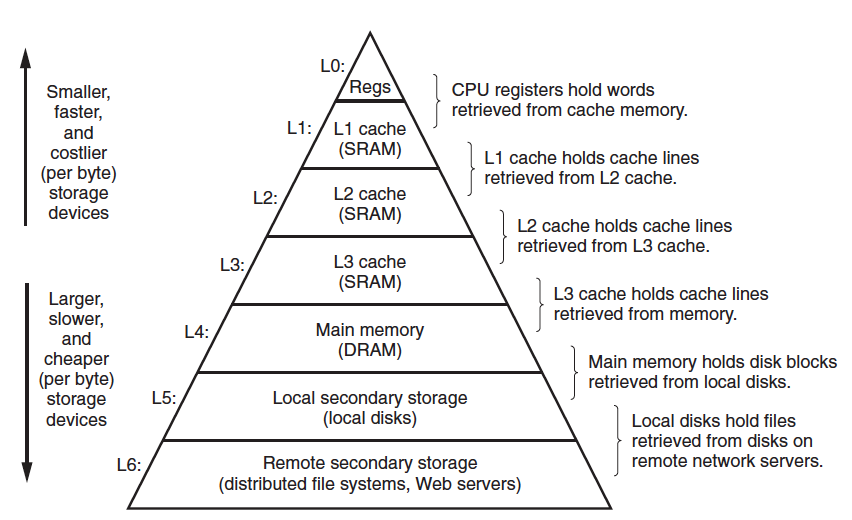
\includegraphics[width=0.99\linewidth]{images/Storage.png}
	\end{figure}
\end{frame}

\begin{frame}
	\frametitle{Architecture of RDBMS, Cont.}
	\begin{columns}
		\column{0.5\textwidth}
		\begin{itemize}
			\item {Query optimization and execution}
			\item Relational operators
			\item Files and access methods
			\item Buffer pool management
			\item Disk space management
		\end{itemize}
		\column{0.5\textwidth}
		\begin{figure}[]
			\includegraphics[width=0.99\linewidth]{images/Arch.png}
		\end{figure}
	\end{columns}
	\pause
	\begin{itemize}
		\item Crash recovery is awfully difficult!
		\begin{itemize}
			\item[$\ast$] The recovery system {\color{red}depends on behavior of many other components} of DBMS, such as concurrency control, buffer management, disk management, and query processing.
		\end{itemize}
	\end{itemize}
\end{frame}


\begin{frame}
	\frametitle{Buffer Pool Management, Cont.}
	\begin{itemize}
		\item {\color{red}Force policy} – make sure that every update is on the DB disk before {\color{red}commit}.
		\begin{itemize}
			\item[\checkmark] Provides durability without REDO logging.
			\item[\checkmark] But, can cause poor performance {\color{blue}due to a large random write operations.}
		\end{itemize}
		\pause
		\item {\color{red}No Steal policy} – don$'$t allow buffer pool frames with uncommited updates to overwrite committed data on DB disk.
		\begin{itemize}
			\item[\checkmark] Useful for ensuring atomicity without UNDO logging.
			\item[\checkmark] But can cause poor performance due to {\color{red}(1)}{\color{blue}A larger buffer is required}; or {\color{red}(2)}{\color{blue} writing that data to temporary location on non-volatile storage (e.g., swap area)}.
		\end{itemize}
	\end{itemize}
	
	\pause
	\fontsize{15pt}{\baselineskip}\selectfont {\color{red} In practice, even to get Force/No-Steal to work requires some nasty details for handling unexpected failures…}
	
\end{frame}

\begin{frame}
	\frametitle{Buffer Pool Replace Policy, Cont.}
	\begin{itemize}
		\item {\color{red}No Force}
		\begin{itemize}
			\item What if system crashes before a modified page written by a committed transaction makes it to DB disk?
			\begin{itemize}
				\item[\checkmark] Write as little as possible, in a convenient place, at commit time, to support REDOing modifications. $\rightarrow$ {\color{red}WAL Logging}.
			\end{itemize}
		\end{itemize}   
		\pause
		\item {\color{red}Steal}
		\begin{itemize}
			\item What if a transaction that performed updates aborts? $\rightarrow$ {\color{red}WAL Logging}
			\item What if system crashes before transaction is finished? $\rightarrow$ {\color{red}WAL Logging}
			\begin{itemize}
				\item[\checkmark] Must remember the old value of P (to support UNDOing the write to page P).
			\end{itemize}
		\end{itemize}
	\end{itemize}
\end{frame}

\begin{frame}
	\frametitle{Buffer Pool Management, Cont.}
	\begin{center}
		
	\end{center}
	\begin{figure}[h]
		\centering
		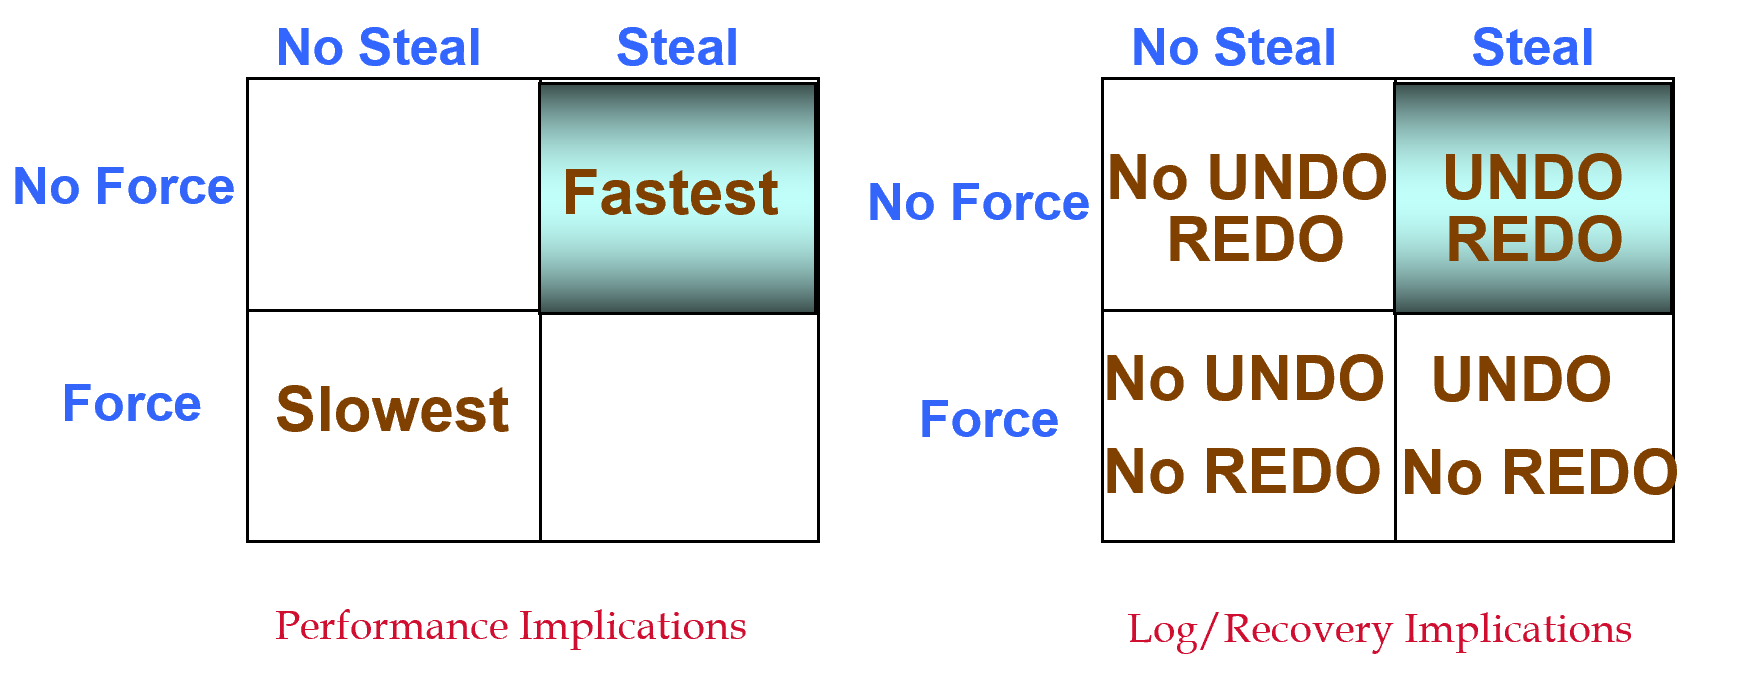
\includegraphics[width=0.99\linewidth]{images/buffer.png}
	\end{figure}    
\end{frame}

\begin{frame}
	\frametitle{Buffer Pool Management, Cont. \footnote[frame]{\href{https://15445.courses.cs.cmu.edu/fall2021/slides/05-bufferpool.pdf}{CMU 15-445/645 Fall 2021 Buffer Pool Slide}}}
	\begin{center}
		
	\end{center}
	\begin{figure}[h]
		\centering
		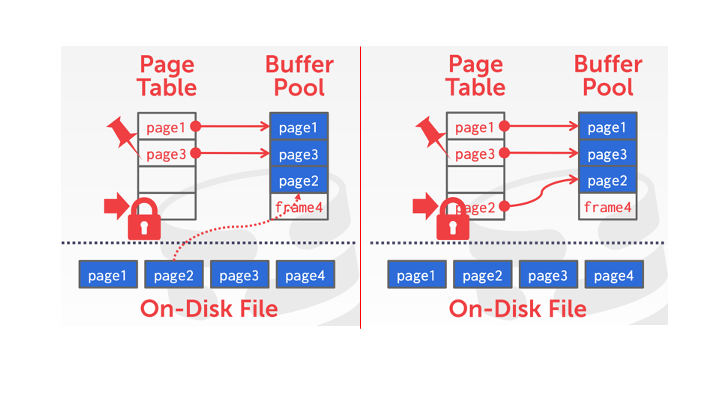
\includegraphics[width=0.95\linewidth]{images/buffer1.png}
	\end{figure}
\end{frame}


\begin{frame}
	\frametitle{MMAP as Buffer Pool, Cont. \footnote[frame]{\href{https://github.com/Ethanzjp/Snippets/tree/master/gendata\_mmap}{Ethanzjp MMAP Gendata Demo}}}
	\begin{itemize}
		\item Memory-mapped (mmap) file I/O is an OS-provided feature.
		\begin{itemize}
			\item<1->[\checkmark] It maps {\color{red}the contents of a file }on secondary storage into a {\color{red}program’s virtual address space}.
			\item<2->[\checkmark] The program then accesses pages via {\color{red}pointers} as if the file resided entirely in memory. 
			\item<3->[\checkmark] The OS {\color{red}transparently loads pages} only when the program references them.
			\item<4->[\checkmark] The OS {\color{red}automatically evicts pages} if memory fills up.
		\end{itemize}
	\end{itemize}
	\pause
	\begin{figure}[h]
		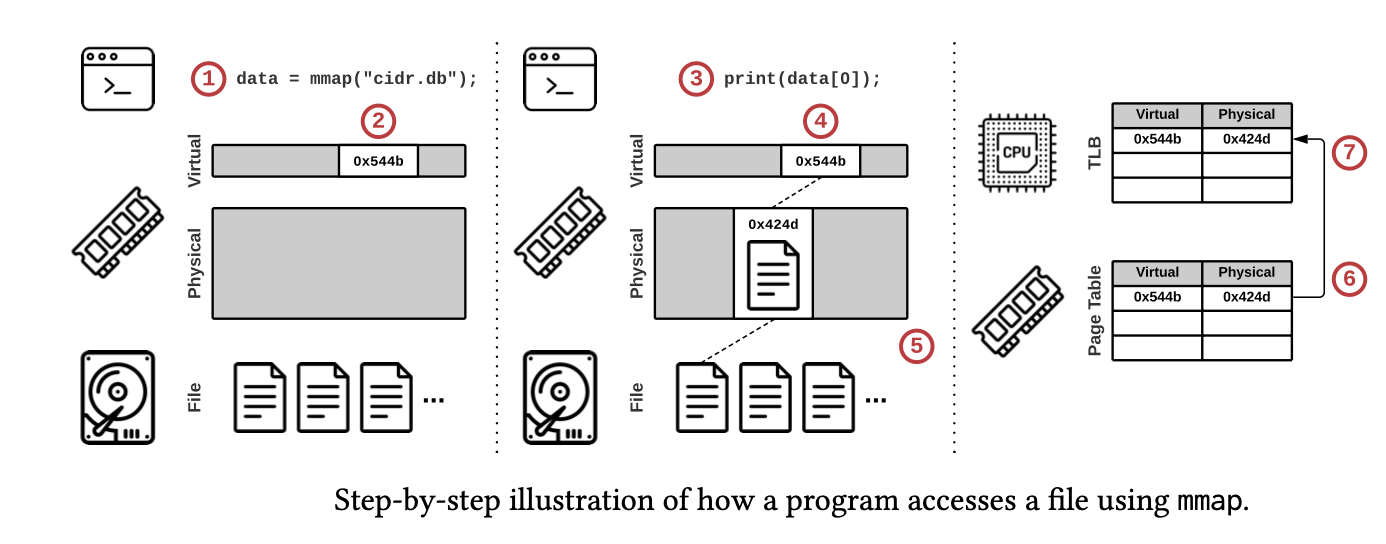
\includegraphics[width=0.75\linewidth]{images/sts.png}
	\end{figure}
\end{frame}

\begin{frame}
	\frametitle{TLB shootdown}
	\begin{itemize}
		\item Shared Memory Model\footnote[frame]{\href{https://github.com/Ethanzjp/Snippets/blob/master/shared\_memory.c}{Ethanzjp Shared Memory Demo}}
		\begin{figure}[h]
			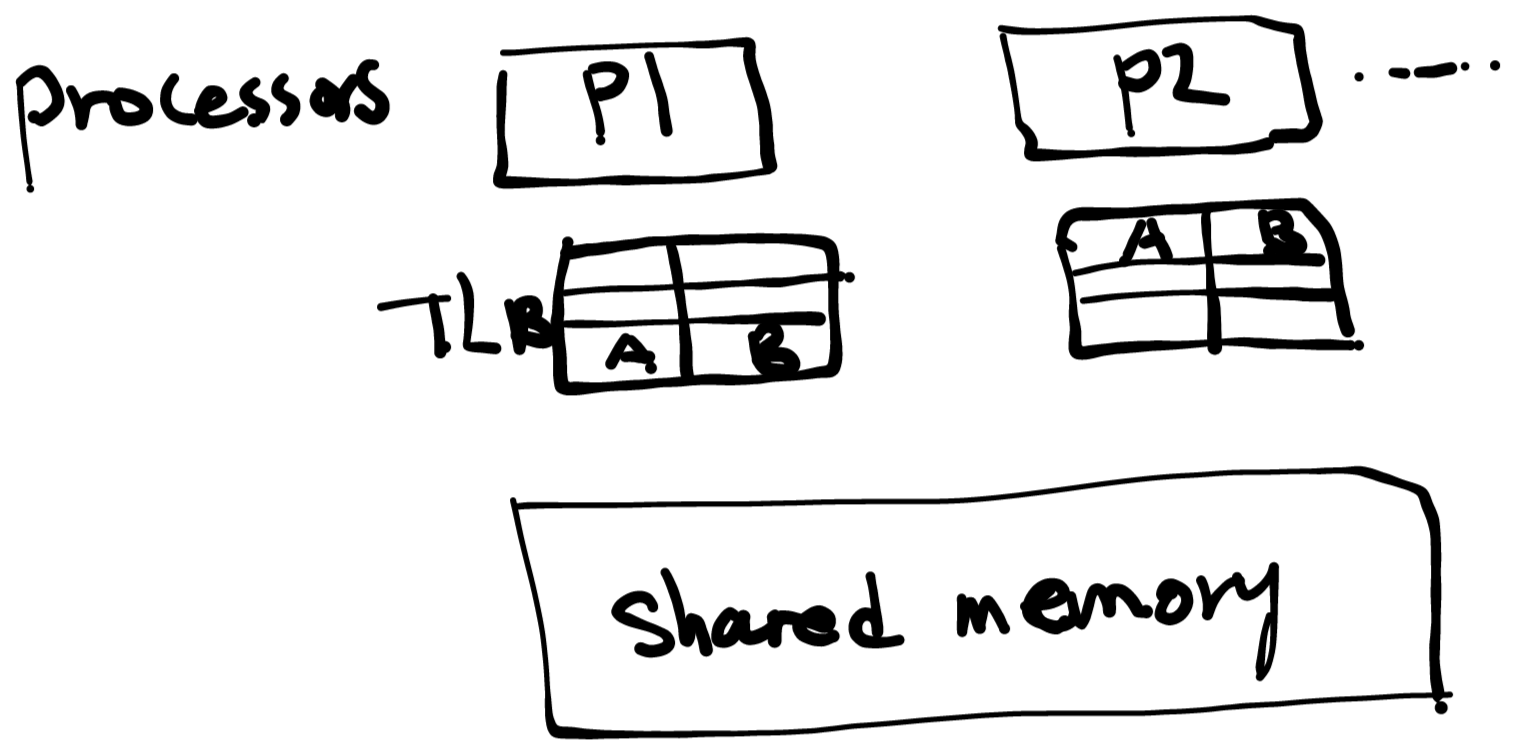
\includegraphics[width=0.75\linewidth]{images/shm.png}
		\end{figure}
	\end{itemize}
\end{frame}

\begin{frame}
	\frametitle{Comparsion of Buffer Pool and MMAP}
	\begin{itemize}
		\item Buffer Pool
		\begin{itemize}
			\item[\checkmark] The DBMS maintaining complete control over how and when it transfers pages. 
		\end{itemize}
		\item MMAP
		\begin{itemize}
			\item[\checkmark] The OS handles all necessary paging behind the scenes rather than the DBMS’s buffer pool. 
		\end{itemize}
		\item Stonebraker 1981 opinion \footnote[frame]{\href{https://citeseerx.ist.psu.edu/viewdoc/download?doi=10.1.1.75.5448&rep=rep1&type=pdf}{1981 Stonebraker's Paper}}
		\begin{figure}[h]
			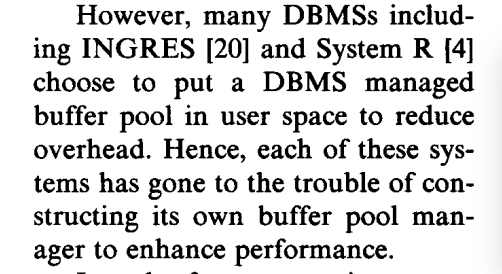
\includegraphics[width=0.50\linewidth]{images/stonebraker.png}
		\end{figure}
	\end{itemize}	
\end{frame}


\begin{frame}
	\frametitle{POSIX API, Cont.}
	\begin{itemize}
		\item mmap \footnote[frame]{\href{https://man7.org/linux/man-pages/man2/mmap.2.html}{mmap man7 page}}
		\item madvise hints to the OS about expected data access patterns\footnote[frame]{\href{https://man7.org/linux/man-pages/man2/madvise.2.html}{madvise man7 page}}
		\begin{figure}[h]
			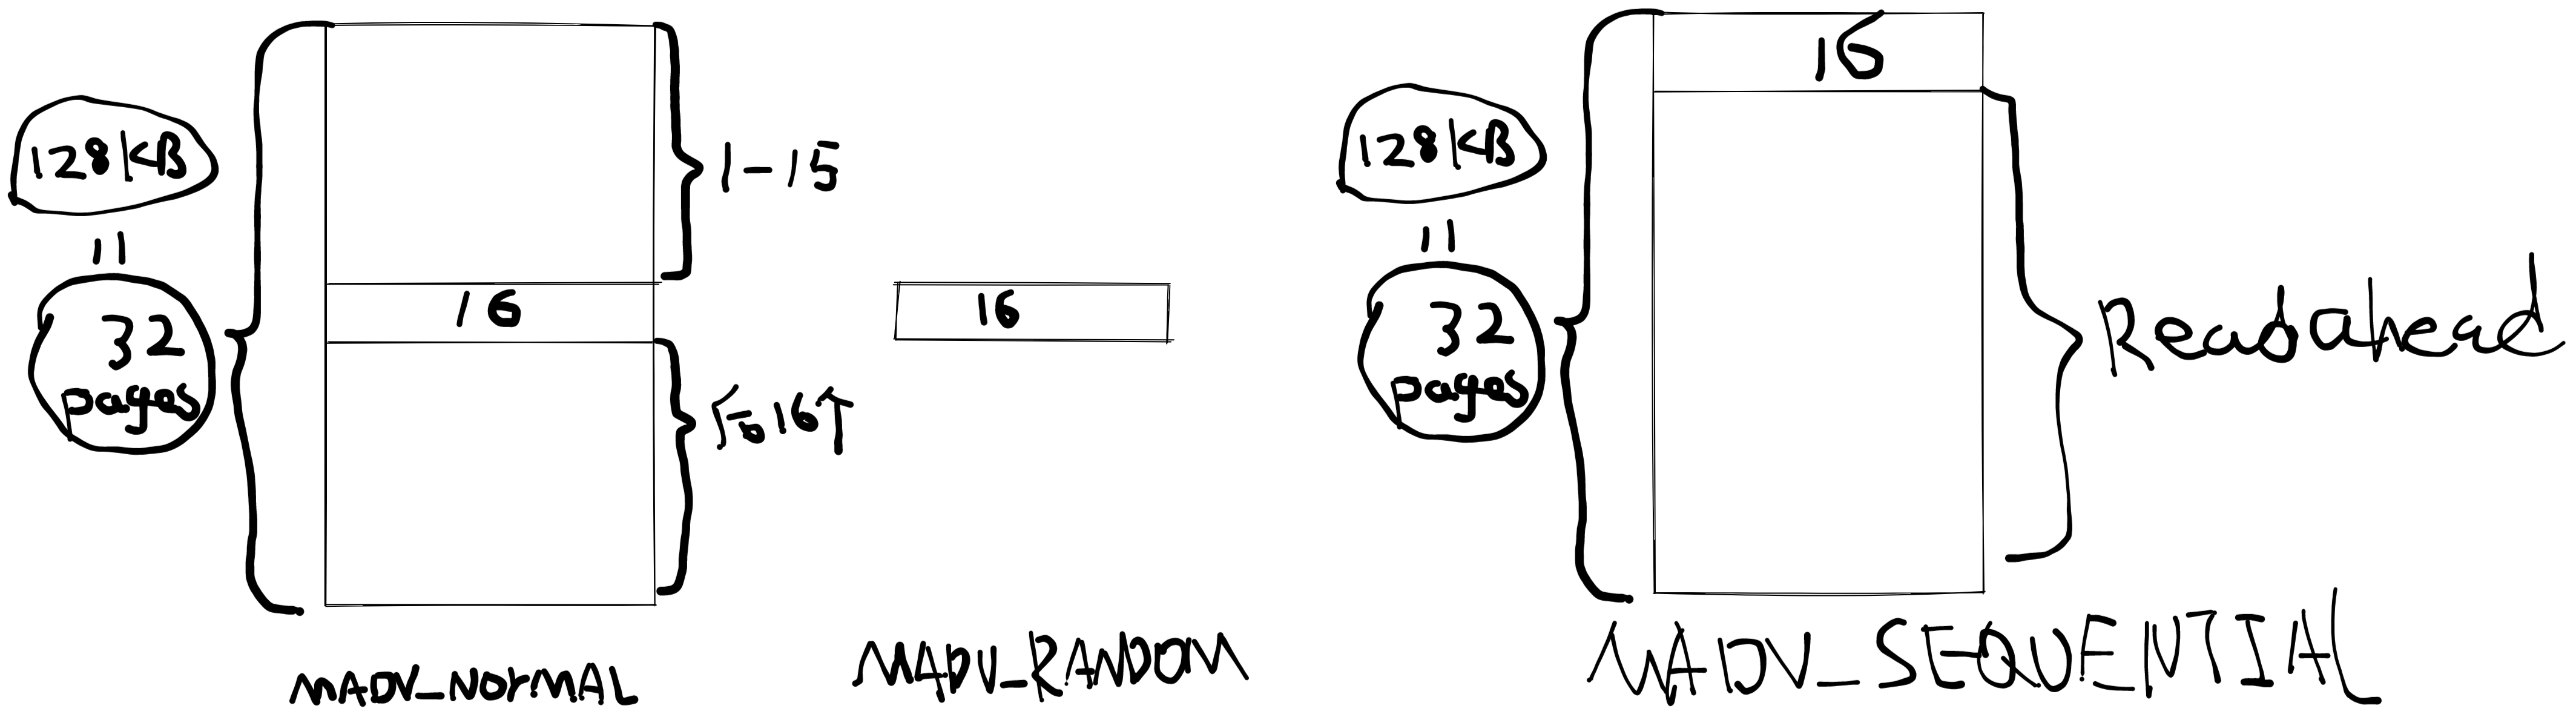
\includegraphics[width=0.99\linewidth]{images/readahead.png}
		\end{figure}
		\item mlock\footnote[frame]{\href{https://man7.org/linux/man-pages/man2/mlock.2.html}{mlock man7 page}} allows DBMS pin memory. {\color{red}But OS is permitted to flush dirty pages to the backing file at any time, even if the page is pinned.}
		\item msync\footnote[frame]{\href{https://man7.org/linux/man-pages/man2/msync.2.html}{msync man7 page}} explicitly flushes the specified memory range to secondary storage.
	\end{itemize}
\end{frame}

\begin{frame}
	\frametitle{Modern MMAP-based DBMS}
	\begin{figure}[h]
		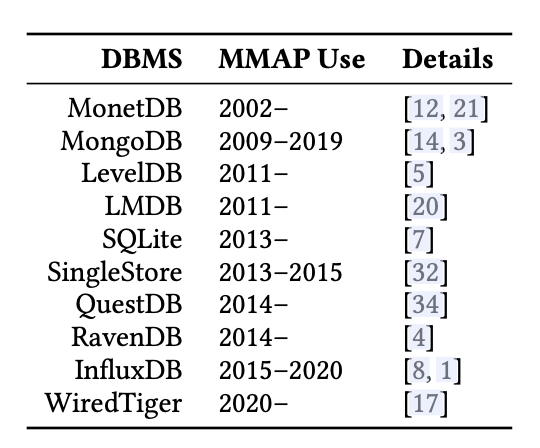
\includegraphics[width=0.35\linewidth]{images/mmap.png}
	\end{figure}
	\pause
	\begin{itemize}
		\item<1-> MonetDB use WiredTiger and MMAPv1 (optional) as storage engine.
		\item<2-> InfluxDB replaced mmap after observing I/O spikes for writes when a database grew larger than a few GB in size.
		\item<3-> SingleStore removed mmap-based file I/O after encountering poor performance on simple sequential scan queries.
		\item<4-> RocksDB replace mmap as a fork of LevelDB
		\footnote[frame]{\href{https://github.com/Ethanzjp/Snippets/tree/master/Level_Snapshot}{LevelDB Snapshot Demo}}.
	\end{itemize}
\end{frame}

\begin{frame}
	\frametitle{What is the truth?}
	\begin{center}
		\fontsize{20pt}{\baselineskip}\selectfont {\color{red}The DBMS seems no longer needs to manage its own buffer pool, as it cedes this responsibility to the OS.  }
	\end{center}
	
\end{frame}

\section{Problem with MMAP: The Four Deadly Sins}
\begin{frame}
	\frametitle{Transactional Safety}
	\begin{itemize}
		\item The challenges inherent with guaranteeing transactional safety of modified pages in mmap-based DBMSs are well-known.
		\begin{itemize}
			\item[$\ast$] Due to transparent paging, {\color{red}the OS can flush a dirty page} to secondary storage {\color{red}at any time}, irrespective of whether the writing transaction has committed. 
			\item[$\ast$] The DBMS cannot prevent these flushes and receives {\color{red}no warning} when they occur.
		\end{itemize}
	\end{itemize}
	\begin{itemize}
		\item Three categories for handling updates:
		\begin{itemize}
			\item<1->[$\ast$] OS CoW
			\begin{itemize}
				\item<2->[\checkmark] MAP\_PRIVATE to enable OS CoW.
				\item<3->[\checkmark]The DBMS modifies the affected pages in the private workspace.
				\item<4->[\checkmark] To provide durability, the DBMS must use a write-ahead log (WAL) to record changes.
				\item<5->[\checkmark] DBMS applies the committed changes to the primary copy using msync.
			\end{itemize}
			\item<6->[$\ast$]  User space CoW
			\begin{itemize}
				\item<7->[\checkmark] Copy the mmap-backed memory page to user buffer.
				\item<8->[\checkmark] Update and recording the WAL logging.
				\item<9->[\checkmark] Copy the modified pages back to the mmap-backed memory.
			\end{itemize}
			\item<10->[$\ast$]  Shadow Paging
		\end{itemize}
	\end{itemize}ß
\end{frame}

\begin{frame}
	\frametitle{System R's Shadow paging}
	\begin{figure}
		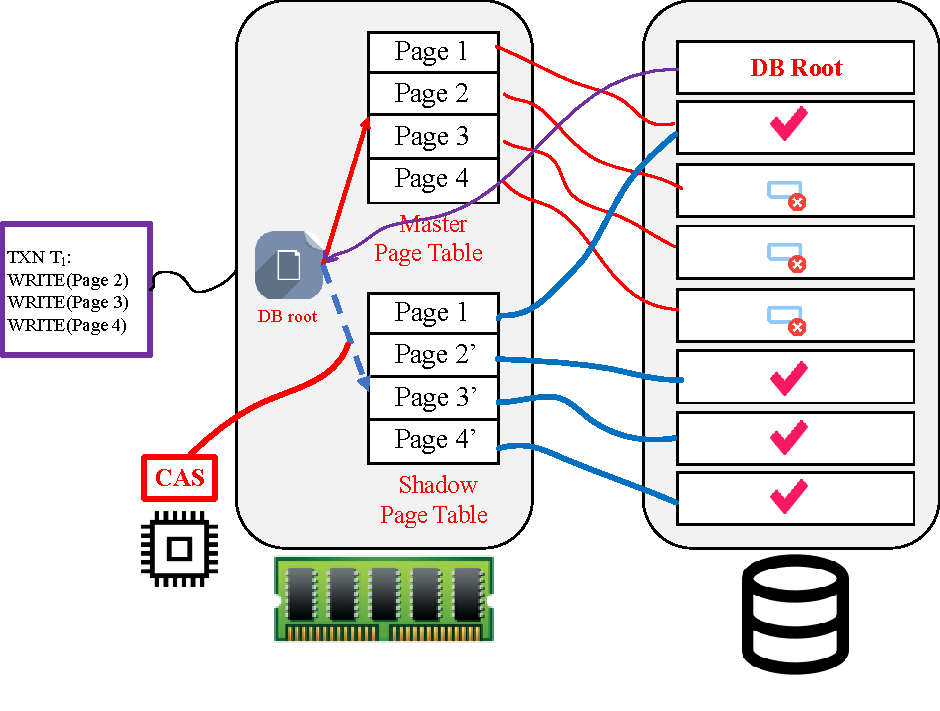
\includegraphics[width=8cm]{images/shadow.pdf}
	\end{figure}
	\begin{itemize}
		\item Master: Contains only changes from committed txns.
		\item Shadow: Temporary db with changes made from uncommitted txns.
	\end{itemize}
\end{frame}

\begin{frame}
	\frametitle{IO Stalls}
	\begin{itemize}
		\item Accessing any page could result in an unexpected I/O stall because the DBMS cannot know whether the page is in memory.
		\begin{itemize}
			\item[\checkmark] Pinning memory.
			\item[\checkmark] mlock the memory.
			\item[\checkmark] madvise, but os is free ignore the advise.
		\end{itemize}
	\end{itemize}
\end{frame}

\begin{frame}
	\frametitle{Error Handling}
	\begin{itemize}
		\item page-level checksums
		\item gracefully handling I/O errors
	\end{itemize}
\end{frame}

\begin{frame}
	\frametitle{Performance Issues}
	\begin{itemize}
		\item page table contention
		\item single-threaded page evictionand for larger-than- memory DBMS workloads on high-bandwidth secondary storage devices.
		\item TLB shootdowns.
		
	\end{itemize}
\end{frame}

\section{Experimental Analysis}
\begin{frame}
	\frametitle{Random Reads on Bandwidth\footnote[frame]{\href{https://github.com/viktorleis/mmapbench}{mmapbenchmark}}}
	\begin{figure}[h]
		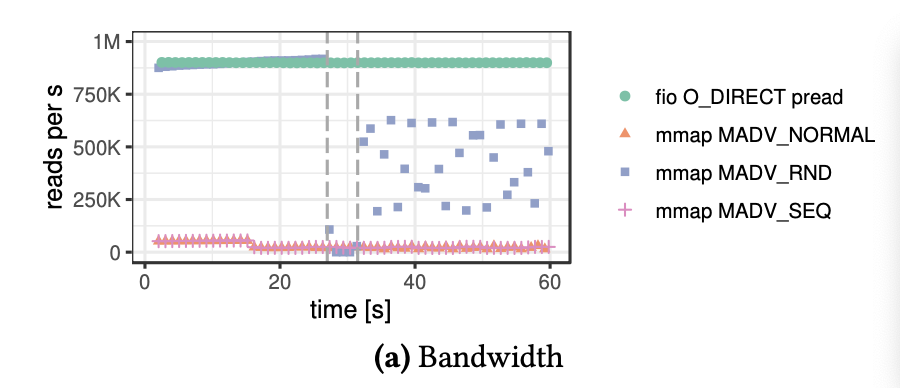
\includegraphics[width=0.75\linewidth]{images/rr.png}
	\end{figure}
	\begin{itemize}
		\item Random access pattern over a 2 TB SSD range to simulate a larger-than-memory OLTP workload.
		\item The page cache had only 100 GB of memory, $95\%$ of all accesses resulted in page faults
		\item fio baseline exhibited stable performance and achieved close to 900K reads per second
	\end{itemize}
\end{frame}

\begin{frame}
	\frametitle{Random Reads on TLB Shootdown}
	\begin{figure}[h]
		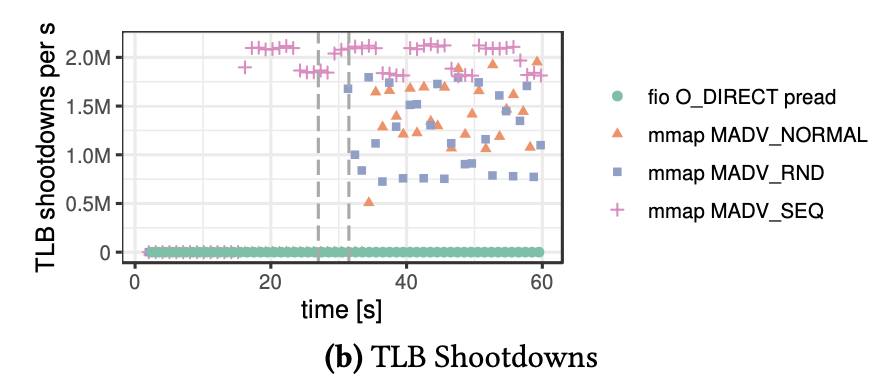
\includegraphics[width=0.75\linewidth]{images/rr_tlb.png}
	\end{figure}
	\begin{itemize}
		\item we measured using /proc/interrupt
	\end{itemize}
\end{frame}

\begin{frame}
	\frametitle{Sequential Scan on Bandwidth}
	\begin{figure}[h]
		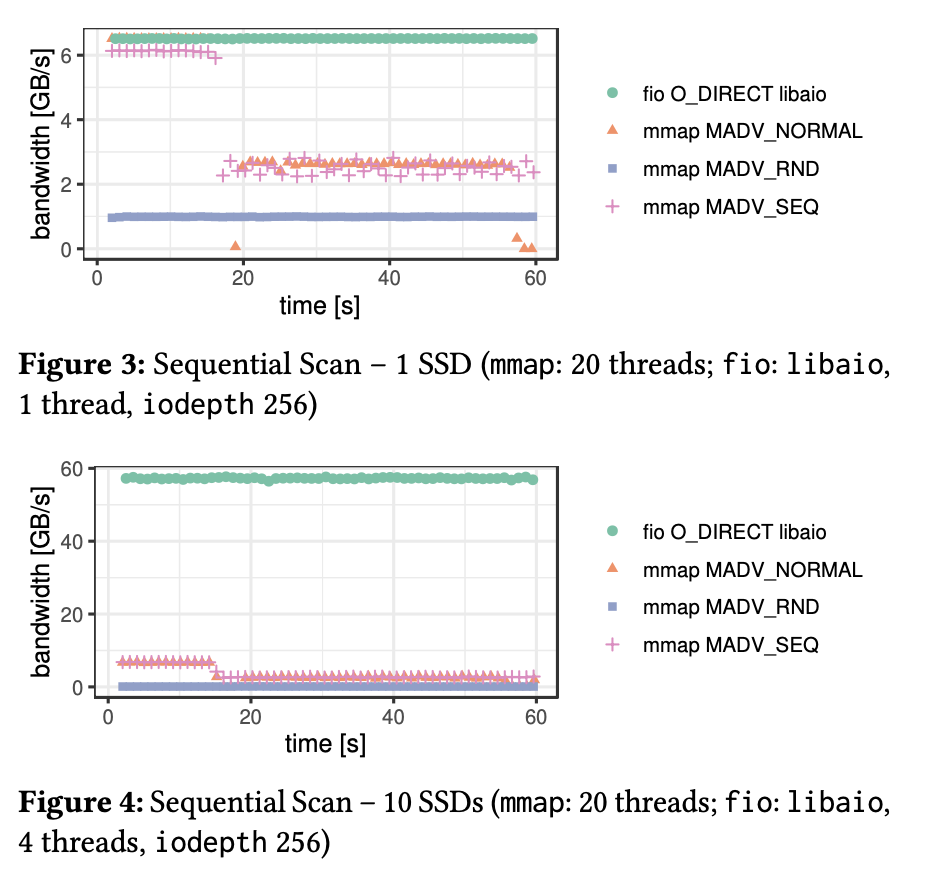
\includegraphics[width=0.65\linewidth]{images/ss.png}
	\end{figure}
\end{frame}

\section{Conclusions}
\begin{frame}
	\frametitle{Conclusions}
	\begin{itemize}
		\item mmap is not a suitable replacement for a traditional buffer pool.
		\item When you should not use mmap in your DBMS:
		\begin{itemize}
			\item<1->[$\ast$] You need to perform updates in a transactionally safe fashion.
			\item<2->[$\ast$] You want to handle page faults without blocking on slow I/O
			or need explicit control over what data is in memory.
			\item<3->[$\ast$] You care about error handling and need to return correc  results.
			\item<4->[$\ast$] You require high throughput on fast persistent storage devices.
		\end{itemize}
		\item<5-> When you should maybe use mmap in your DBMS:
		\begin{itemize}
			\item<6->[\checkmark] Your working set (or the entire database) fits in memory and
			the workload is read-only.
			\item<7->[\checkmark] You need to rush a product to the market and do not care about
			data consistency or long-term engineering headaches.
			\item<8->[\checkmark] Otherwise, never.
		\end{itemize}
		
	\end{itemize}
\end{frame}

\section{References}
\begin{frame}
	\frametitle{References}
	\begin{thebibliography}{1234567891011}
		\bibitem {1} \href{https://ravendb.net/articles/re-are-you-sure-you-want-to-use-mmap-in-your-database-management-system}{RavenDB Response}
		\bibitem{2} \href{https://news.ycombinator.com/item?id=29936104}{Community Comments}
	\end{thebibliography}
\end{frame}

\section{Acknowledgements and Questions}
\begin{frame}
	\frametitle{}
	\begin{center}
		Thank you! \\
		Welcome for any questions!
	\end{center}
	\begin{figure}
		
\includegraphics[width=2cm]{images/thanks.png}
	\end{figure}
	\frametitle{}
	\begin{center}
		Junpeng Zhu \\
		% crimezjp@foxmail.com \\
		Greenplum, VMware, Inc.
	\end{center}
\end{frame}

\end{document}